\chapter{Príklady úloh do súťaží}
\label{kap:CTF}

V tejto kapitole využijeme výsledky analýzy útokov z kapitoly \ref{kap:utoky} na prípravu ukážkových úloh do súťaží. Podarilo sa nám demonštrovať, že pomocou útoku využívajúceho techniku zmeny napätia vieme spôsobiť cielené vynechanie inštrukcie. Na útok využijeme zapojenie s tranzistorom, ktoré bolo pre naše účely dostatočne účinné. Zároveň budeme brať do úvahy obmedzenie dané nízkou rýchlosťou hardvéru riadiaceho obvod s tranzistorom. Kritickú časť kódu, na ktorú bude v príklade treba zacieliť preto implementujeme v asembleri a inštrukcie zvolíme tak, aby bolo útok možné úspešne realizovať.

Konkrétne uvedieme dva príklady, jeden základný cielene implementovaný tak, aby bolo jednoduché na program zaútočiť. V druhom príklade sa budeme snažiť uviesť realistickejší program, ktorý udeľuje prístup pomocou čítačky RFID (Radio Frequency IDentification) kariet. Následne demonštrujeme úspešný útok, ktorý spôsobí, že program udelí prístup aj po prečítaní karty, ktorej prístup nemal udeliť. Súčasťou oboch príkladov bude zároveň vzorové riešenie, v ktorom popíšeme použitý program aj potrebné zapojenie pre realizáciu útoku. Pri riešení oboch príkladoch využijeme znalosť zdrojového kódu programu. (Zdrojové kódy programov z oboch príkladov sú dostupné v elektronickej prílohe priloženej k prác.) V reálnej situácii by pravdepodobne pred implementáciou útoku bolo potrebné skompilovaný kód analyzovať pomocou reverzného inžinierstva a nájsť v kóde citlivé inštrukcie, na ktoré zacieliť. Takáto analýza však presahuje rámec tejto práce a našim zámerom je demonštrovať funkčnosť samotného útoku. V elektronickej prílohe sa nachádzajú . V elektronickej prílohe sa však nachádzajú aj skompilované HEX obrazy oboch programov, ktoré možno priamo nahrať na útokom cielený mikrokontrolér ATMega328P, napríklad pomocou softvéru AVRDUDE \cite{avrdude}.

\section{Príklad 1 -- Uzamknutý čip} \label{kap4:sek:priklad1}
Ako prvý predstavíme jednoduchý príklad podobný s príkladom zo súťaže CTF, na ktorý sme útočili v sekcii \ref{kap3:sek:utokNaFirmverCTF}. Cieľom tohto príkladu bude ukázať niektoré základné princípy postupu pri útoku pomocou indukovania chýb -- identifikovať citlivú časť kódu, využitie výstupných signálov programu na synchronizáciu zdroja útoku s cieľom a správne načasovanie útoku.

Najskôr je potrebné spojazdniť program, na ktorý následne budeme útočiť. Program využíva na výstup dve signalizačné LED a sériovú komunikáciu pomocou rozhrania UART. Okrem základného zapojenia mikrokontroléra z obrázku \ref{obr:schemeATMega} teda pripojíme cez 330 $\Omega$ odpor ešte dve LED -- červenú k pinu GPIO 7 (Port D7) a zelenú k pinu GPIO 8 (Port B0). Schéma celého zapojenia aj s útočiacim hardvérom je na obrázku \ref{obr:schemeCTF-LED}. Následne nahráme program na cieľový mikrokontrolér ATMega328P. Po spustení program po chvíli na sériový port pošle správu, že čip úspešne naštartoval. Následne začne periodicky blikať červenou LED a posielať správu \uv{čip je v stave uzamknutý}. Zadaním tejto úlohy je teda \uv{odomknúť} čip.

\subsection{Vzorové riešenie}
Po analýze zdrojového kódu zistíme, že hlavný beh programu sa skladá z dvoch while-cyklov. V prvom sa mení logická hodnota na porte červenej LED (čo spôsobuje efekt blikania) a periodicky sa posiela správa \uv{čip je v stave uzamknutý}. Pričom prvý cyklus sa opakuje kým premenná \uv{status} bude rovná nule. Po skončení prvého cyklu sa rozsvieti zelená LED (bit v príslušnom porte sa nastaví na logickú jednotku) a následne sa spustí druhý cyklus v ktorom sa periodicky posiela správa \uv{čip je v stave odomknutý}. Ukážka  popísaných častí kódu je v algoritme \ref{alg:mainCTF1}. Cieľom nášho útoku bude teda spôsobiť, aby sa prvý cyklus ukončil.

\begin{lstlisting}[float,language=C,caption={Ukážka kóu hlavnej časti programu z príkladu 1.},label=alg:mainCTF1]
// 1. while-cyklus (status je globálna premenná typu uint8_t)
while(!status) {
    Serial.println("Chip status: locked"); // výpis na sériový port
    digitalWrite(RED_LED, HIGH); // zapnutie červnej LED
    checkStatus(); // táto funkcia pristupuje k premennej status
    delay(500);
    digitalWrite(RED_LED, LOW); // vypnutie červnej LED
    delay(500);
}

digitalWrite(RED_LED, LOW); // vypnutie červnej LED
digitalWrite(GREEN_LED, HIGH); // zapnutie zelenej LED

// 2. while-cyklus (cieľom je, aby sa sem program dostal)
while(1) {
    Serial.println("Chip status: unlocked"); // výpis na sériový port
    delay(1000);
}
\end{lstlisting}

To možno vo všeobecnosti (pomocou indukovania chýb) dosiahnuť rôznymi spôsobmi, napr. ovplyvnením inštrukcie skoku, zápisu do premennej \uv{status}. Nie všetky ovplyvnenia sú však jednoducho dosiahnuteľné najmä pri použití lacnejšieho hardvéru ako sme ukázali v kapitole \ref{kap:utoky}. Možno si však všimnúť, že v prvom cykle sa opakuje volanie funkcie \uv{checkStatus}, ktorá pristupuje ku kľúčovej premennej \uv{status}. Následne sa spustí časť kódu písaná v asembleri -- séria tridsiatich inštrukcií, ktoré modifikujú aj register, ktorého výsledná hodnota sa následne uloží do premennej \uv{status}. (Previazanie častí kódu písaných v jazykoch C a asembler je zabezpečené vďaka C Inline Assembly \cite{inlineAsm}.) Ukážky úryvkov kódu z funkcie \uv{checkStatus} sú v algoritme \ref{alg:asmCTF1}. Sémantika tejto časti programu vyzerá na prvý pohľad krypticky -- nepravidelné striedanie zdanlivo náhodných inštrukcií, ktoré modifikujú registre. Po hlbšej analýze napríklad prekopírovaním inštrukcií do emulátora architektúry AVR a dynamickej analýze jeho správania zistíme, že sled inštrukcií je zvolený tak, aby výsledok bol vždy rovnaký -- v registri previazaným s premennou \uv{status} bude uložená hodnota nula. To spôsobí, že program beží dookola v prvom cykle.

\begin{lstlisting}[float,language=AVR,caption={Ukážky kritickej časti kódu funkcie \uv{checkStatus} z príkladu 1. \%0 označuje výstupný parameter -- register s výstupnou hodnotou. Tento parameter je previazaný s globálnou premennou status pomocou C Inline Assembly \cite{inlineAsm}.},label=alg:asmCTF1]
; inicializácia registrov
ldi %0, 0xFF
ldi r24, 0x20
ldi r25, 0x0F
ldi r26, 0xAA

; začiatok kódu, ktorý manipuluje s registrami
mov r3, r26
dec %0
add %0, r24
sub %0, r25
or %0, r26
add r26, r25
add %0, r26
clr r26         ; inštrukcia clr vynuluje register
sub r26, r24
eor %0, r3      ; inštrukcia xor v architektúre AVR

; ...

; záver
ldi r25, 0x2F
or %0, r25
inc %0 ; v registri pod týmto parametrom bude výstupná hodnota
\end{lstlisting}

Postupnosť inštrukcií bola zámerne zvolená tak, aby zásah do (takmer) každej inštrukcie spôsobil, že výsledok už nebude rovný nule. Táto časť kódu je preto pomerne citlivá na útok pomocou indukovania chýb -- vynechanie ľubovolnej inštrukcie z tejto časti s vysokou pravdepodobnosťou spôsobí, že výsledkom už nebude hodnota nula a program prejde do druhého cyklu, čím sa čip odomkne. Aby to bolo možné dosiahnuť, je potrebné riadenie útoku správne načasovať. Pre mierne sťaženie úlohy sú navyše niektoré inštrukcie zámerne \uv{zbytočné} a ich vynechanie neovplyvní výsledok. Pre načasovanie útoku možno využiť samotný program bežiaci na cieli. Tesne pred zavolaním funkcie \uv{checkStatus} sa volá funkcia, ktorá zapína červenú LED. Tento výstup možno využiť ako signál pre synchronizáciu. Zároveň bude treba útok od prijatia signálu správne načasovať tak, aby sa trafil do kritickej časti kódu. Navyše, ako bolo spomenuté, niektoré inštrukcie nemajú vplyv na výsledok. Preto ich vynechanie výsledok neovplyvní a útok bude neúspešný. Napriek tomu bude načasovanie pomerne jednoduché. Necielime totiž na konkrétnu inštrukciu, ale stačí trafiť (takmer) ktorúkoľvek inštrukciu v rámci funkcie \uv{checkStatus}.

Využijeme teda útok pomocou techniky zmeny napätia, konkrétne zapojenie s tranzistorom, ktorý sme analyzovali v sekcii \ref{kap3:sek:analyZaTranzistoru}. Ako riadiaci hardvér zvolíme dosku Arduino Nano a využijeme aj rovnaký program zo sekcie \ref{kap3:sek:testovanieEfektov} v kapitole \ref{kap:utoky}, bude však treba upraviť parameter posun. Program nastavíme tak, aby začal s hodnotou posunu jeden a postupne ju bude zväčšovať po každom pokuse o útok o jeden. V sekcii \ref{kap3:sek:testovanieEfektov} sme pozorovali, že pri doske Arduino Nano predstavoval posun hodnoty jeden približne 200 ns. Maximálnu hodnotu parametra posun môžeme preto nastaviť napríklad na desať čo predstavuje dve mikrosekundy (10 $\cdot$ 200 ns). V sekcii \ref{kap3:sek:testovanieEfektov} sme ďalej odhadli priemernú dĺžku jednej inštrukcie (na cieľovom ATMega328P) na približne 1/16 \textmu s. Dve mikrosekundy posunu teda predstavujú približne 32 inštrukcií, čo zďaleka presahuje potrebné oneskorenie pre zásah do citlivej časti kódu. Nastavenie väčšej hodnoty posunu už nemá preto veľký zmysel. Po dosiahnutí maximálnej hodnoty parametra posun sa táto hodnota obnoví na jeden a takto bude program pokračovať až kým sa útok nepodarí. Schéma zapojenia aj s doskou Nano, ktorá riadi útok je na obrázku \ref{obr:schemeCTF-LED}.

\begin{figure}
    \centerline{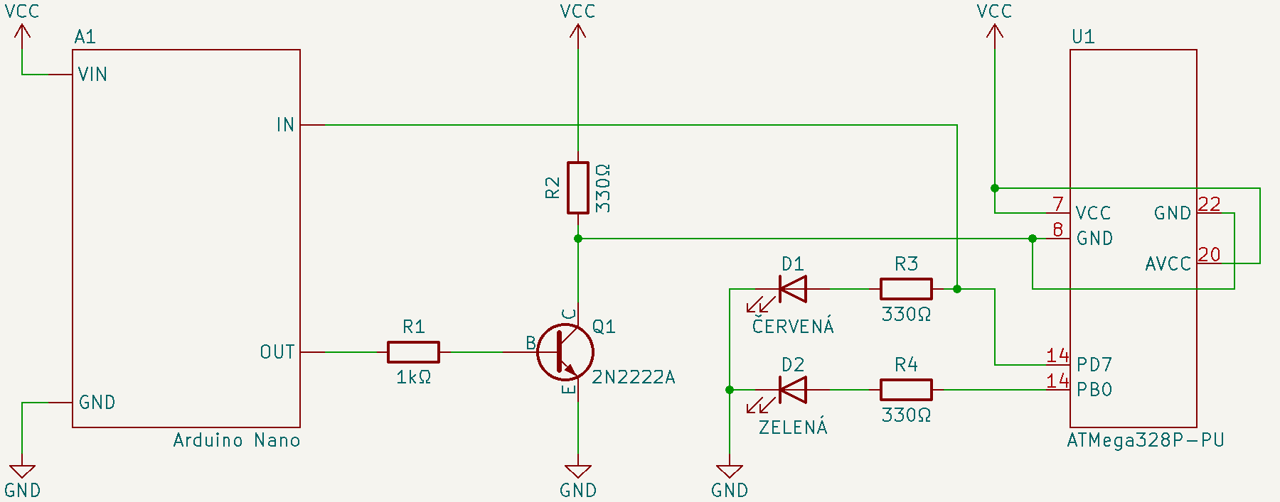
\includegraphics[width=1\textwidth]{images/schemeCTF-LED.png}}
    \caption[Schéma zapojenia pre útok na príklad 1]{Schéma zapojenia pre útok na príklad 1 -- Uzamknutý čip. K mikrokontroléru ATMega328P sú pripojené aj ostatné komponenty (nie sú znázornené kvôli prehľadnosti) podľa schémy \ref{obr:schemeATMega} z kapitoly \ref{kap:hardver}.}
    \label{obr:schemeCTF-LED}
\end{figure}

Popísaný postup sme následne implementovali a útok sa podarilo úspešne realizovať. Útok bol úspešný hneď pri hodnote jeden parametra posun. Program rozsvietil zelenú LED a začal posielať správu \uv{čip je v stave odomknutý}. Pri hodnote parametra posun viac ako jeden bol útok už neúspešný (posun bol pravdepodobne príliš dlhý). V prípade, že by sme útok riadili pomocou dosky Discovery, postup by bol analogický. Akurát by bolo opäť potrebné správne nastaviť parameter posun. Pravdepodobne na väčšiu hodnotu, keďže doska Discovery má väčšiu frekvenciu procesora. Keďže na úspešný útok postačovala doska Nano, dosku Discovery sme v tomto príklade nepoužili. Riadenie útoku oboma doskami sme pre naše účeli dostatočne porovnali pri analýze v kapitole \ref{kap:utoky}.

\section{Príklad 2 -- Čítačka RFID kariet} \label{kap4:sek:priklad2}
Druhým príkladom je program, ktorý udeľuje prístup na základe čítačky RFID (Radio Frequency Identification) kariet, ďalej len čipová karta. Cieľom tohto príkladu je demonštrácia útoku na realistickejší program v porovnaní s prvým príkladom. Inšpiráciu programu na čítanie čipových kariet sme prevzali z ročníkového projektu Deadlock \cite{deadlock}. Program sme pre naše účely do značnej mieri zjednodušili. Pôvodný program predstavuje čítačku kariet, ktorá zároveň komunikuje so serverom a na základe tejto komunikácie sa rozhoduje, či udelí prístup. Z programu sme odstránili komunikáciu so serverom a rozhodnutie o udelení prístupu sme \uv{zadrôtovali} do programu porovnaním s konštantou. Toto porovnanie sme implementovali v jazyku asembler spôsobom, aby bolo jednoduchšie na program zaútočiť. Túto časť kódu bližšie analyzujeme vo vzorovom riešení.

Zároveň bolo potrebné modifikovať zapojenie hardvéru, keďže pôvodný program nebol implementovaný pre mikrokontrolér ATMega328P. Pre zapojenie hardvéru budú potrebné nasledovné komponenty:
\begin{itemize}
    \item ATMega328P-PU -- THT púzdro
    \item kontaktné bez-spájkové pole
    \item modul PN532 pre čítanie RFID kariet pomocou NFC (Near Field Communication) -- zapojíme cez rozhranie SPI (Serial Peripheral Interface)
    \item rezistory -- 4-krát 330 $\Omega$ k LED
    \item 4 kusy LED -- rôzne farby (červená, zelená, žltá, biela)
    \item prepojovacie kábliky typu M-M (Male to Male)
    \item všetky ostatné súčiastky použité v základnom zapojení mikrokontroléra ATMega328P zo sekcie \ref{kap2:sek:zakladneZapojenie}.
\end{itemize}
Najskôr zapojíme základné komponenty k mikrokontroléru podľa zapojenia z obrázku \ref{obr:schemeATMega} z kapitoly \ref{kap:hardver}. Ostatné časti doplníme podľa zapojenia na obrázku \ref{obr:schemeRFID}. Toto zapojenie ešte neobsahuje hardvér potrebný pre útok, ale predstavuje korektné zapojenie pre fungovanie programu.

\begin{figure}
    \centerline{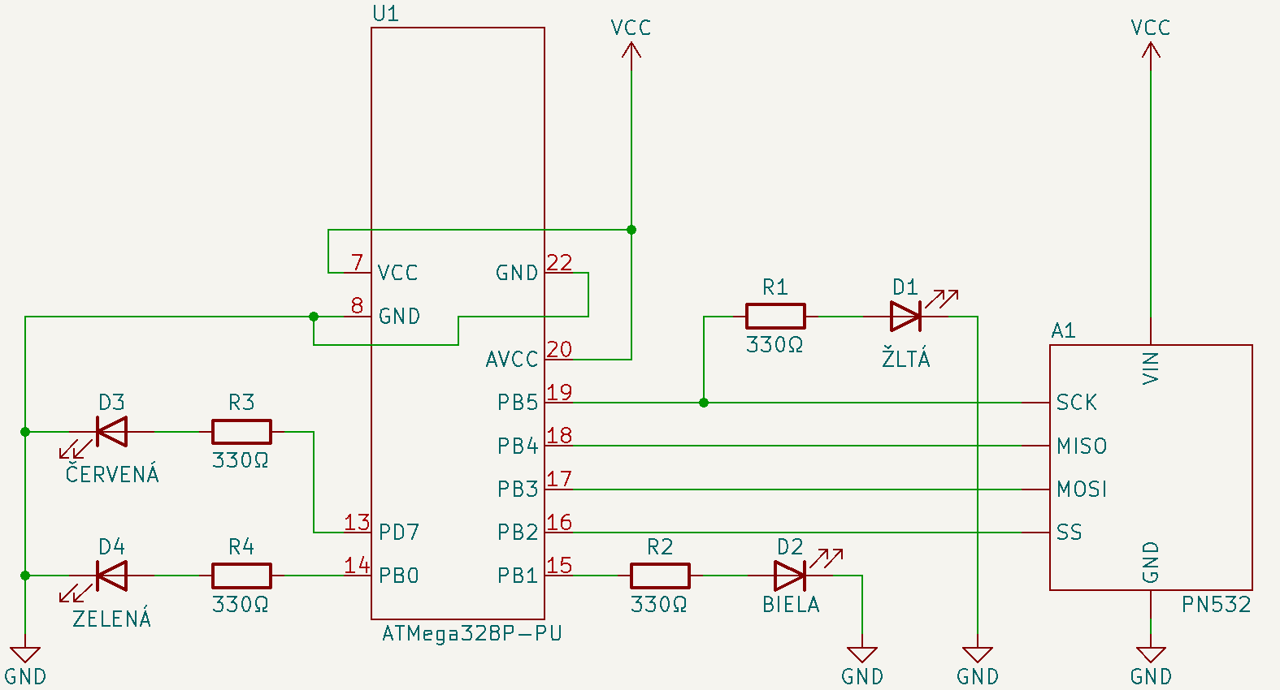
\includegraphics[width=1\textwidth]{images/schemeRFID.png}}
    \caption[Schéma zapojenia mikrokontroléra v príklade 2]{Schéma zapojenia mikrokontroléra v príklade 2 -- Čítačka RFID kariet. Okrem znázorneného zapojenia sú k mikrokontroléru pripojené aj základné súčiastky z obrázku \ref{obr:schemeATMega}. (Zapojenie žltej LED sme pre jednoznačnosť uviedli aj v tomto obrázku.)}
    \label{obr:schemeRFID}
\end{figure}

Teraz môžeme nahrať a spustiť program na cieľovom ATMega328P. Po spustení program, pošle správu na sériový port, že bol úspešne naštartovaný. V prípade, že sa nepodarí nadviazať komunikáciu s modulom PN532 pre čítanie RFID kariet, program pošle chybovú hlášku. Pokiaľ nastane tento problém, pravdepodobne ide o nesprávne zapojenie hardvéru. Pokiaľ všetko prebehne správne, spustí sa hlavný cyklus, v ktorom sa program pokúsi prečítať čipovú kartu podľa štandardu ISO14443A. Pokiaľ čítačka žiadnu čipovú kartu nedeteguje, pošle na sériový port správu, že čaká na priloženie karty. Tento proces sa periodicky opakuje. Po priložení karty a úspešnom prečítaní, sa na krátku chvíľu rozsvieti biela LED na indikáciu, že čítanie bolo úspešné. Následne sa rozsvieti červená alebo zelená LED, ktorá indikuje zamietnutie, resp. povolenie prístupu, zároveň program pošle príslušnú správu na sériový port. Program je nastavený tak, aby udelil prístup jedinej čipovej karte a to karte s konkrétnym UID (Unique Identifier) rovným 0x348BD1A3 (v poradí od najvýznamnejšieho bajtu). Zadaním tejto úlohy je pomocou indukovania chýb prinútiť mikrokontrolér, aby udelil prístup (indikované rozsvietením zelenej LED) po prečítaní karty s nesprávnym ID, ktorej prístup nemal udeliť.

\subsection{Vzorové riešenie}
Opäť bude prvým krokom analýza zdrojového kódu. Keďže zdrojový kód príkladu 2 je mierne rozsiahlejší, pre podrobnosti ohľadom popisovaných častí kódu odkazujeme čitateľa do elektronickej prílohy, v ktorej sa nachádza kompletný (príslušne okomentovaný) zdrojový kód (cesta k adresáru: {\color{olive} /CTFexamples/CTF-RFID/}). Podstatné časti kódu však popíšeme aj v práci.

Rozhodnutie o udelení prístupu program urobí na základe návratovej hodnoty (typu bool) funkcie \uv{checkAccess}. Hlavná časť funkcie \uv{checkAccess} je napísaná v jazyku asembler (s využitím C Inline Assembly \cite{inlineAsm}). Ako prvé funkcia nastaví návratovú hodnotu na nulu (prístup zamietnutý). Zároveň vynuluje register R0. Následne sa spustí séria porovnaní, bajt po bajte, medzi UID prečítaným z priloženej čipovej karty (v registroch) a staticky definovaným UID karty, ktorej má byť prístup udelený. Jedno porovnanie pozostáva zo samotného porovnania registra s konštantou a podmieneného skoku, ktorý preskočí práve jednu inštrukciu v prípade rovnosti. Inštrukcia, ktorú skok preskočí je inkrement registra R0, ktorý sa tým pádom vykoná iba v prípade, že porovnanie skončilo nenulovým výsledkom. Ukážka tejto časti kódu v jazyku asembler je v algoritme \ref{alg:asmCTF2}. Týmto spôsobom sa porovná najskôr dĺžka prečítaného UID (podľa štandardu ISO14443A môže UID mať dĺžku štyri alebo sedem bajtov) a následne najmenej významné štyri bajty prečítaného UID. 

\begin{lstlisting}[float,language=AVR,caption={Ukážky kódu v asembleri z funkcie \uv{checkAccess} z príkladu 2. \%0 označuje výstupný parameter. Ostatné parametre (označené \%) sú argumentami jednotlivých inštrukcií CPI. CPI porovná vždy register -- prečítaný bajt UID a konštantu -- bajt UID \uv{správnej kary} (staticky deklarovaný).},label=alg:asmCTF2]
; inicializácia - vynulovanie registrov
clr %0
eor r0, r0

; porovnania prvého bajtu (dĺžka UID)
cpi %1, %2      ; porovnanie prečítanej dĺžky UID
breq skip_1     ; podmienený skok ak nastala rovnosť
inc r0          ; inkrement registra R0

; porovnania druhého bajtu (prvý bajt UID)
skip_1:         ; návestie pred ďalším porovnaním
cpi %3, %4      ; porovnanie prvého bajtu UID
breq skip_2     ; podmienený skok ak nastala rovnosť
inc r0          ; inkrement registra R0

skip_2:         ; návestie pred ďalším porovnaním
; ...

; ...
breq skip_5     ; podmienený skok po poslednom porovnaní
inc r0          ; inkrement registra R0

skip_5:         ; návestie pred záverečným testom R0
tst r0          ; test na nulu registra R0

; na túto inštrukciu cielime útok:
brne fail       ; podmienený skok ak R0 bol nenulový

ldi %0, 0x01    ; uloženie hodnoty 1 do výstupu
fail:
nop             ; posledná inštrukcia v asembleri

; nasleduje návrat z funkcie (už v jazyku C)
\end{lstlisting}

Pokiaľ všetky porovnania skončili nulovým výsledkom (rovnosť) v registry R0 zostane inicializovaná hodnota nula, v opačnom prípade bude R0 obsahovať nenulovú hodnotu (aspoň jeden inkrement sa vykoná). Na záver sa vykoná test na nulu registra R0, pokiaľ bola hodnota nulová do registra obsahujúceho návratovú hodnotu funkcie sa zapíše hodnota jeden (čo znamená \uv{prístup povolený}). V prípade, že by priložená karta mala UID dĺžky inej ako štyri bajty, nebudú sa rovnať dĺžky, teda prvé porovnanie skončí nenulovou hodnotou a prístup nebude udelený. Dôvodom prečo algoritmus porovnania neskončí hneď pri prvej nerovnosti je znemožnenie útoku postranným kanálom, konkrétne časovým útokom (angl. timing attack). Popísaná implementácia má tú vlastnosť, že porovnanie trvá rovnako nezávisle od počtu rovných bajtov.

Nevýhodou však je, že výsledok celého porovnania závisí na jednom podmienenom skoku (po záverečnom teste registra R0). Pokiaľ sa tento skok nevykoná návratová hodnota z funkcie bude jeden a prístup bude udelený. Táto inštrukcia je potom vhodný cieľ nášho útoku. Zároveň hneď pred zavolaním funkcie \uv{checkAccess}, na ktorú chceme útok zacieliť, je v programe volanie funkcie \uv{digitalWrite}, ktorá rozsvieti bielu LED. Pomocou tohto signálu môžeme, rovnako ako v príklade 1, synchronizovať útok s cieľovým mikrokontrolérom.

Opäť budeme na program útočiť pomocou zapojenia s tranzistorom, z kapitoly \ref{kap:utoky}. Keďže budeme cieliť na konkrétnu inštrukciu, tentokrát bude útok riadený pomocou dosky Discovery, o ktorej sme ukázali, že poskytuje väčšiu presnosť ako doska Nano. Zapojenie útočiaceho hardvéru je podobné ako v príklade 1, jeho schéma je na obrázku \ref{obr:schemeCTF-RFID}. Pre posielanie správ o nastavených parametrov útoku z dosky Discovery do počítača sme pripojili ďalší prevodník z USB na UART (rovnaký model ako v zapojení z obrázku \ref{obr:schemeATMega}), podobne ako pri útoku v sekcii \ref{kap3:sek:testovanieEfektov}. Program pre riadenie útoku bude opäť rovnaký ako v sekcii \ref{kap3:sek:testovanieEfektov} (program pre dosku Discovery). Analogicky ako v príklade 1 zo sekcie \ref{kap4:sek:priklad1}, bude potrebné nastaviť rozsah parametra posun, ktorý sa bude s každým pokusom automaticky inkrementovať. Rozsah parametra posun sme nastavili od jeden po sto. V kapitole \ref{kap:utoky} sme zistili, že doska Discovery je približne o jeden rád presnejšia ako doska Nano.

\begin{figure}
    \centerline{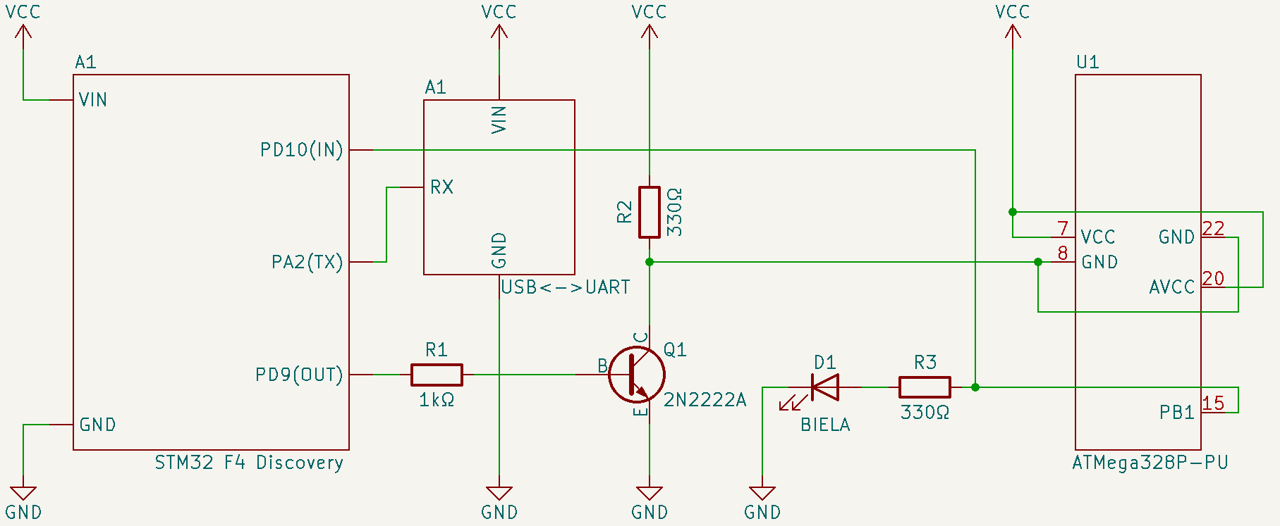
\includegraphics[width=1\textwidth]{images/schemeCTF-RFID.png}}
    \caption[Schéma zapojenia pre útok na príklad 2]{Schéma zapojenia pre útok na príklad 2 -- Čítačka RFID kariet. Opäť, kvôli prehľadnosti, nie sú znázornené súčiastky zo zapojení \ref{obr:schemeATMega} a \ref{obr:schemeRFID}, ktoré je tiež potrebné k ATMega328P pridať. (Zapojenie bielej LED sme pre jednoznačnosť uviedli aj v tomto obrázku.)}
    \label{obr:schemeCTF-RFID}
\end{figure}

Útok sme implementovali podľa uvedeného postupu. Po postupnom prikladaní čipovej karty (s UID, ktorému program nemá povoliť prístup) k čítačke sa zakaždým spustil útok riadený doskou Discovery. Útok bol synchronizovaný na základe signálu, ktorý vyslal cieľový mikrokontrolér tým, že po priložení karty rozsvietil bielou LED na upozornenie, že úspešne prečítal čipovú kartu. Po každom pokuse o útok doska Discovery automaticky zväčšila parameter posun až kým sa úspešne podarilo dosiahnuť, aby mikrokontrolér zasvietil zelenou LED a zároveň poslal správu \uv{prístup povolený}, napriek tomu, že priložená karta nemala mať povolený prístup. (UID bolo rôzne od 0x348BD1A3 čo je jediné, ktorému program udelí prístup.) Hodnoty parametra posun, pri ktorých sa útok úspešne podaril boli 31 a 32. Pri menšej, alebo väčšej hodnote buď program prístup zamietol (bez známok poruchy), alebo zlyhal a mikrokontrolér sa reštartoval.

Následne sme sa pokúsili útok zopakovať riadením pomocou dosky Nano. Tentokrát bol však útok neúspešný pre všetky hodnoty parametra posun v rozmedzí 1 -- 20. Väčšie hodnoty nemalo zmysel skúšať, keďže rádovo presahujú očakávané časove oneskorenie od prijatia signálu po vykonanie cieľovej inštrukcie.